
\chapter{HASIL DAN PEMBAHASAN}


% Jelaskan Proses Implementasi 
\section{Implementasi pada FPGA Development Board}

Pada penelitian ini digunakan 6 kernel berbeda berukuran 3x3 untuk penerapan filter spasial linear pada video \textit{stream} 720p 60 FPS. Penerapan tersebut dilakukan pada FPGA Development Board yang menggunakan prosesor ARM dan pada FPGA Development Board yang sama menggunakan FPGA. Kemudian dilakukan analisis kinerja dari keduanya untuk menunjukan masing-masing waktu komputasi, FPS, penggunaan CPU, penggunaan \textit{memory}, \textit{resident memory} (RES), \textit{shared memory} (SHR), dan \textit{virtual memory} (VIRT).

FPGA Development Board dirangkai seperti yang telah disebutkan di Bab sebelumnya, dapat dilihat pada gambar \ref{fig:rancangan-sistem}. HDMI Output pada FPGA dihubungkan ke monitor dan HDMI Input dihubungkan ke \textit{source} dalam hal ini Laptop Lenovo Ideapad 320. FPGA Development Board juga dihubungkan ke \textit{router} menggunakan kabel UART agar dapat diakses menggunakan protokol \textit{ssh}. Selanjutnya memasang semua \textit{library} yang dibutuhkan di FPGA Development Board.
% \subsection{Representasi Video Stream sebagai Citra Digital}
% \subsection{Konversi Frame menjadi Grayscale}
\subsection{Penerapan Filter Spasial}
Setiap frame dari \textit{source} video \textit{stream} dibaca sebagai matriks berukuran 1280x720 dengan rentang nilai keabuan pada masing-masing piksel yaitu dari 0 sampai 255. Setiap piksel pada matriks tersebut hanya memiliki satu lapis warna karena citra yang diterima dari source adalah citra \textit{grayscale}, tidak seperti citra warna yang memiliki tiga lapis warna pada setiap pikselnya. 
% padding?

Proses filter spasial dilakukan dengan operasi konvolusi pada setiap matriks dengan kernel yang telah ditentukan sebelumnya. Operasi konvolusi ini menghasilkan matrix baru dengan ukuran 1280x720. Matriks hasil tersebut selanjutnya direpresentasikan kembali sebagai citra digital yang selanjutnya disebut sebagai hasil filter. Hasil filter dari setiap frame ini ditampilkan ke monitor melalui HDMI Output pada FPGA Development Board secara berkesinambungan sehingga tampak seperti video.

\begin{afigure}
    \includegraphics[width=0.8\linewidth, center]{images/output-image/input1-grayscale.png}
    \caption{Contoh Frame Grayscale.}
    \label{fig:input-grayscale}
\end{afigure}

Salah satu contoh frame dari \textit{source} dapat dilihat pada gambar \ref{fig:input-grayscale}. Selanjutnya dilakukan filter spasial menggunakan 6 kernel yang telah ditentukan sebelumnya.

\subsubsection{Average Blur}
Penerapan filter spasial pada frame \textit{grayscale} yang berukuran 1280x720 pixel dengan kernel \textit{average blur} (\ref{kernel:average}) yang berukuran 3x3 menghasilkan cita blur yang berukuran 1280x720. Hasil filter \textit{average blur} dapat dilihat pada gambar \ref{fig:output-averageblur}. Filter seperti ini dapat digunakan untuk mengurangi derau pada citra.
\begin{afigure}
    \includegraphics[width=0.8\linewidth, center]{images/output-image/input1-averageblur.png}
    \caption{Hasil filter Average Blur.}
    \label{fig:output-averageblur}
\end{afigure}

\subsubsection{Gaussian Blur}
Penerapan filter spasial dengan kernel \textit{gaussian blur} (\ref{kernel:gaussianblur}) yang berukuran 3x3 menghasilkan cita blur yang secara kasat mata mirip dengan filter \textit{average blur}. Namun apabila diperhatikan nilai masing-masing pixel pada gambar \ref{fig:output-gaussianblur} akan terlihat perbedaan dengan nilai masing-masing pixel pada gambar \ref{fig:output-averageblur}. Hal ini disebabkan oleh nilai bobot pada kernel \textit{gaussian blur} (\ref{kernel:gaussianblur}) yang berbeda dengan kernel \textit{average blur} sehingga hasil konvolusinya juga berbeda. 
\begin{afigure}
    \includegraphics[width=0.8\linewidth, center]{images/output-image/input1-gaussianblur.png}
    \caption{Hasil filter Gaussian Blur.}
    \label{fig:output-gaussianblur}
\end{afigure}

\subsubsection{Laplacian}
Penerapan filter spasial dengan kernel \textit{laplacian} (\ref{kernel:laplacian}) menghasilkan cita biner yang hanya direpresentasikan dengan warna hitam dan putih saja, dapat dilihat pada gambar \ref{fig:output-laplacian}. Filter seperti ini dapat digunakan pada metode deteksi tepi dalam proses pengolahan citra digital.
\begin{afigure}
    \includegraphics[width=0.8\linewidth, center]{images/output-image/input1-laplacian.png}
    \caption{Hasil filter Laplacian.}
    \label{fig:output-laplacian}
\end{afigure}

\subsubsection{Sharpening}
Penerapan filter spasial dengan kernel \textit{sharpening} (\ref{kernel:sharpen}) dapat meningkatkan detail (seperti garis) pada citra, namun dapat juga dapat menimbulkan derau pada citra apabila nilai kernelnya tidak sesuai. Filter seperti ini lebih tepat digunakan untuk memperbaiki kualitas citra (dengan nilai kernel yang sesuai). Hasil filter \textit{sharpening} ini dapat dilihat pada gambar \ref{fig:output-sharpen}.
\begin{afigure}
    \includegraphics[width=0.8\linewidth, center]{images/output-image/input1-sharpen.png}
    \caption{Hasil filter Sharpening.}
    \label{fig:output-sharpen}
\end{afigure}

\subsubsection{Sobel Horizontal}
Penerapan filter spasial dengan kernel \textit{sobel horizontal} (\ref{kernel:sobel}) menghasilkan cita biner, dapat dilihat pada gambar \ref{fig:output-sobelhor}. Filter seperti lebih tepat digunakan pada metode deteksi tepi di citra yang banyak mengandung garis horizontal.
\begin{afigure}
    \includegraphics[width=0.8\linewidth, center]{images/output-image/input1-sobelhor.png}
    \caption{Hasil filter Sobel Horizontal.}
    \label{fig:output-sobelhor}
\end{afigure}

\subsubsection{Sobel Vertical}
Penerapan filter spasial dengan kernel \textit{sobel vertical} (\ref{kernel:sobel}) menghasilkan cita biner, dapat dilihat pada gambar \ref{fig:output-sobelver}. Sama halnya dengan filter \textit{sobel horizontal}, filter \textit{sobel vertical} juga dapat digunakan untuk metode deteksi tepi, terutama pada citra yang banyak mengandung garis verikal.
\begin{afigure}
    \includegraphics[width=0.8\linewidth, center]{images/output-image/input1-sobelver.png}
    \caption{Hasil filter Sobel Vertical.}
    \label{fig:output-sobelver}
\end{afigure}

\subsection{Penerapan Filter Spasial menggunakan Prosesor ARM dan FPGA}
Penerapan filter spasial menggunakan prosesor ARM dilakukan dengan menggunakan \textit{library} OpenCV dengan bahasa pemrograman Python yang dijalankan pada FPGA Development Board. Sedangkan untuk penerapan filter spasial menggunakan FPGA dilakukan dengan menggunakan \textit{library} xfOpenCV dari Xilinx. \textit{Library} xfOpenCV ini adalah library khusus yang dimodifikasi dari OpenCV sehingga proses komputasinya dapat dilakukan dengan FPGA, bukan dengan prosesor ARM yang pada FPGA Development Board ini. Lebih lanjut mengenai program yang digunakan dapat dilihat pada lampiran \textit{pynq-filter-spasial-arm} dan \textit{pynq-filter-spasial-fpga}.

\subsection{Proses Evaluasi Kinerja}
Pada penelitian ini peneliti melakukan dua proses dalam evaluasi kinerja. Proses pertama untuk menghitung waktu komputasi dan FPS dari masing-masing kernel dengan prosesor ARM dan FPGA. Kemudian proses kedua untuk mencatat penggunaan CPU dan penggunaan memory termasuk \textit{resident memory}, \textit{shared memory} dan \textit{virtual memory}. 

\subsubsection{Menghitung Waktu Komutasi dan FPS}
Pada proses ini peneliti melakukan percobaan dengan menggunakan 50 frame dan 200 frame dari \textit{source} untuk dihitung FPS dan waktu komputasinya. Percobaan dilakukan sebanyak 5 kali menggunakan 50 frame untuk masing-masing kernel pada prosesor ARM dan FPGA, dan 5 kali percobaan menggunakan 200 frame untuk masing-masing kernel. Hasil masing-masing percobaan ini dapat dilihat pada lampiran (?).

Menghitung waktu komputasi dilakukan dengan cara mencatat waktu mulai dan waktu semua frame selesai difilter pada setiap percobaan. Waktu komputasi diperoleh dari selisih antara waktu selesai dengan waktu mulai. Dilakukan dengan 50 frame dan 200 frame pada masing-masing kernel menggunakan prosesor ARM dan FPGA. Proses ini dilakukan dengan menggunakan \textit{library time} pada bahasa pemrograman Python, dapat dilihat pada gambar \ref{code:calculate-time}.
\begin{afigure}
    \lstinputlisting[frame=single, style=python]{images/programs/calculate-time.py}
    \caption{Menghitung waktu komputasi dengan library time di Python.}
    \label{code:calculate-time}
\end{afigure}

Hasil waktu komputasi ini dicatat dan kemudian digunakan untuk menghitung FPS dari masing-masing percobaan. FPS masing-masing percobaan ini dihitung dengan menggunakan persamaan \ref{eq:fps}.

\subsubsection{Mencatat Penggunaan Memory dan CPU (Resource)}
Pada proses ini peneliti menggunakan program bawaan dari Linux yang berjalan di FPGA Development Board untuk membantu mencatat penggunaan memory dan CPU (\textit{resource}) pada saat proses penerapan filter spasial. Program ini menampilkan data tentang proses yang berjalan seperti ID sebuah proses, berapa persen memory yang digunakan oleh sebuah proses, persentase CPU yang digunakan, berapa lama sebuah proses berjalan, \textit{resident memory}, \textit{shared memory} dan \textit{virtual memory}. Contoh output program tersebut dapat dilihat pada gambar \ref{fig:top-linux}.
\begin{afigure}
    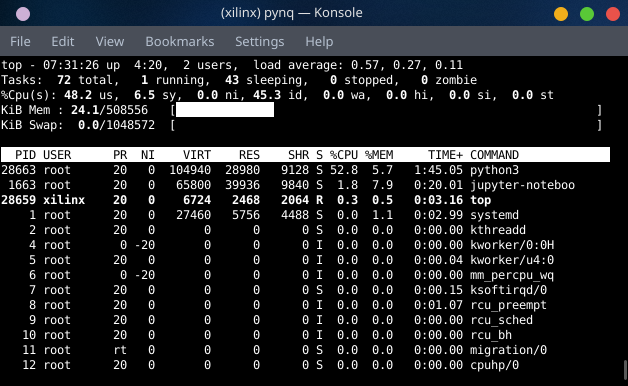
\includegraphics[width=0.8\linewidth, center]{images/programs/top-linux.png}
    \caption{Tampilan program \textbf{top}.}
    \label{fig:top-linux}
\end{afigure}

Peneliti melakukan 5 kali percobaan untuk mencatat penggunaan memory dan CPU dari masing-masing kernel dengan prosesor ARM dan FPGA. Percobaan implementasi ini menggunakan Jupyter Notebook yang berjalan di FPGA Development Board yang dapat diakses menggunakan Web Browser dari perangkat lain. Serta digunakan protokol SSH untuk mengakses FPGA Development Board dan menjalankan program untuk menampilkan penggunaan \textit{resource} dari proses yang sedang berjalan.

\begin{afigure}
    \lstinputlisting[frame=single, style=python]{images/programs/pid.py}
    \caption{Menampilkan PID sebuah proses dengan bahasa pemrograman Python.}
    \label{code:pid}
\end{afigure}

Pertama peneliti menampilkan ID proses dari Jupyter Notebook yang digunakan untuk percobaan mencatat penggunaan memory dan CPU dari penerapan filter menggunakan prosesor ARM dan FPGA. Cara menampilkan ID proses (PID) menggunakan bahasa pemrograman Python dapat dilihat pada gambar \ref{code:pid}. ID proses tersebut kemudian digunakan pada program \textbf{top} untuk menampilkan \textit{resource} yang digunakan pada saat tersebut. 

\begin{afigure}
    \begin{lstlisting}[frame=single, style=shell] 
    $ top -d 0.1 -p 4382 -b >> arm-laplacian1.txt    
    \end{lstlisting}
    \caption{Menjalankan program \textbf{top} kemudian menyimpan hasilnya pada file arm-laplacian1.txt.}
    \label{code:top}
\end{afigure}

Pada gambar \ref{code:top} ditunjukan cara menggunakan program \textbf{top} untuk mencatat penggunaan \textit{resource} dari proses dengan ID 4382 kemudian \textit{output}nya disimpan di file \textit{arm-laplacian1.txt}. Program \textbf{top} tersebut dijalankan sesaat sebelum proses penerapan filter dijalankan pada Jupyter Notebook. Output dari program top setiap 0.1 detik disimpan pada file text yang telah ditentukan. Setelah seluruh frame selesai difilter maka program \textbf{top} juga dihentikan.

\begin{afigure}
    \lstinputlisting[frame=single, style=plain]{images/programs/arm-laplacian1.txt}
    \caption{Potongan isi file arm-laplacian1.txt.}
    \label{code:arm-laplacian1.txt}
\end{afigure}

Isi file \textit{arm-laplacian1.txt} setelah program selesai dijalankan dapat dilihat pada gambar \ref{code:arm-laplacian1.txt}. Isi dari file hasil ini masih banyak mengandung informasi yang tidak dibutuhkan pada penelitian ini, sehingga perlu dilakukan proses ekstraksi informasi yang dibutuhkan saja. Kemudian file yang telah diekstraksi tersebut dibuat menjadi file CSV agar lebih mudah dalam proses pengolahan selanjutnya, seperti pada gambar \ref{code:arm-laplacian1.csv}. Proses tesebut dilakukan sebanyak 5 kali percobaan pada masing-masing kernel menggunakan prosesor ARM dan FPGA.

\begin{afigure}
    \lstinputlisting[frame=single, style=plain]{images/programs/arm-laplacian1.csv}
    \caption{Isi file arm-laplacian1.csv.}
    \label{code:arm-laplacian1.csv}
\end{afigure}

% Jelaskan Hasil
\section{Analisis Kinerja}
\subsection{Waktu Komuptasi}
\begin{atable}
    \caption{Tabel perbandingan waktu komputasi dengan menggunakan 50 frame.}
    \label{table:hasil-time50}
    \csvreader[
        head to column names,
        tabular=lcc,
        separator=semicolon,
        before table=\rowcolors{2}{gray!15}{gray!30},
        table head= \rowcolor{gray!50!black} 
            \color{white} Filter & 
            \color{white} Prosesor ARM (s) & 
            \color{white} FPGA (s)\\]
        {tables/hasil-time50.csv}
        {
            filter=\filter, 
            arm=\arm, 
            fpga=\fpga}
        {
            \filter & 
            \arm & 
            \fpga }
\end{atable}
\blindtext
\begin{afigure}
    \includegraphics[width=0.9\linewidth, center]{images/chart/chart-time50.png}
    \caption{Grafik perbandingan waktu komputasi dengan menggunakan 50 frame.}
    \label{fig:chart-time50}
\end{afigure}


\subsection{Frame Rate (FPS)}
\blindtext
\begin{atable}
    \caption{Tabel perbandingan FPS dengan menggunakan prosesor ARM dan FPGA.}
    \label{table:hasil-fps}
    \csvreader[
        head to column names,
        tabular=lcc,
        separator=semicolon,
        before table=\rowcolors{2}{gray!15}{gray!30},
        table head= \rowcolor{gray!50!black} 
            \color{white} Filter & 
            \color{white} Tanpa FPGA & 
            \color{white} Dengan FPGA \\]
        {tables/hasil-fps.csv}
        {
            filter=\filter, 
            arm=\arm, 
            fpga=\fpga}
        {
            \filter & 
            \arm & 
            \fpga }
\end{atable}
\begin{afigure}
    \includegraphics[width=0.9\linewidth, center]{images/chart/chart-time50.png}
    \caption{Grafik perbandingan FPS dengan menggunakan 50 frame.}
    \label{fig:chart-fps50}
\end{afigure}

\subsection{Penggunaan CPU}
\begin{atable}
    \caption{Tabel perbandingan penggunaan CPU dengan menggunakan prosesor ARM dan FPGA.}
    \label{table:hasil-cpu}
    \csvreader[
        head to column names,
        tabular=lcc,
        separator=semicolon,
        before table=\rowcolors{2}{gray!15}{gray!30},
        table head= \rowcolor{gray!50!black} 
            \color{white} Filter & 
            \color{white} Prosesor ARM (\%) & 
            \color{white} FPGA (\%)\\]
        {tables/hasil-cpu.csv}
        {
            filter=\filter, 
            arm=\arm, 
            fpga=\fpga}
        {
            \filter & 
            \arm & 
            \fpga }
\end{atable}
\blindtext
\begin{afigure}
    \includegraphics[width=0.9\linewidth, center]{images/chart/chart-cpu.png}
    \caption{Grafik perbandingan penggunaan CPU dengan menggunakan prosesor ARM dan FPGA.}
    \label{fig:chart-cpu}
\end{afigure}

\subsection{Penggunaan Memory}
\begin{atable}
    \caption{Tabel perbandingan penggunaan memory dengan menggunakan prosesor ARM dan FPGA.}
    \label{table:hasil-mem}
    \csvreader[
        head to column names,
        tabular=lcc,
        separator=semicolon,
        before table=\rowcolors{2}{gray!15}{gray!30},
        table head= \rowcolor{gray!50!black} 
            \color{white} Filter & 
            \color{white} Prosesor ARM (\%) & 
            \color{white} FPGA (\%)\\]
        {tables/hasil-mem.csv}
        {
            filter=\filter, 
            arm=\arm, 
            fpga=\fpga}
        {
            \filter & 
            \arm & 
            \fpga }
\end{atable}
\blindtext
\begin{afigure}
    \includegraphics[width=0.9\linewidth, center]{images/chart/chart-mem.png}
    \caption{Grafik perbandingan penggunaan memory dengan menggunakan prosesor ARM dan FPGA.}
    \label{fig:chart-mem}
\end{afigure}

\subsection{Resident Memory (RES)}
\begin{atable}
    \caption{Tabel perbandingan penggunaan resident memory dengan menggunakan prosesor ARM dan FPGA.}
    \label{table:hasil-res}
    \csvreader[
        head to column names,
        tabular=lcc,
        separator=semicolon,
        before table=\rowcolors{2}{gray!15}{gray!30},
        table head= \rowcolor{gray!50!black} 
            \color{white} Filter & 
            \color{white} Prosesor ARM (KiB) & 
            \color{white} FPGA (KiB)\\]
        {tables/hasil-res.csv}
        {
            filter=\filter, 
            arm=\arm, 
            fpga=\fpga}
        {
            \filter & 
            \arm & 
            \fpga }
\end{atable}
\blindtext
\begin{afigure}
    \includegraphics[width=0.9\linewidth, center]{images/chart/chart-res.png}
    \caption{Grafik perbandingan penggunaan resident memory dengan menggunakan prosesor ARM dan FPGA.}
    \label{fig:chart-res}
\end{afigure}

\subsection{Shared Memory (SHR)}
\begin{atable}
    \caption{Tabel perbandingan penggunaan shared memory dengan menggunakan prosesor ARM dan FPGA.}
    \label{table:hasil-shr}
    \csvreader[
        head to column names,
        tabular=lcc,
        separator=semicolon,
        before table=\rowcolors{2}{gray!15}{gray!30},
        table head= \rowcolor{gray!50!black} 
            \color{white} Filter & 
            \color{white} Prosesor ARM (KiB) & 
            \color{white} FPGA (KiB)\\]
        {tables/hasil-shr.csv}
        {
            filter=\filter, 
            arm=\arm, 
            fpga=\fpga}
        {
            \filter & 
            \arm & 
            \fpga }
\end{atable}
\blindtext

\begin{afigure}
    \includegraphics[width=0.9\linewidth, center]{images/chart/chart-shr.png}
    \caption{Grafik perbandingan penggunaan shared memory dengan menggunakan prosesor ARM dan FPGA.}
    \label{fig:chart-shr}
\end{afigure}

\subsection{Virtual Memory (VIRT)}
\begin{atable}
    \caption{Tabel perbandingan penggunaan virtual memory dengan menggunakan prosesor ARM dan FPGA.}
    \label{table:hasil-virt}
    \csvreader[
        head to column names,
        tabular=lcc,
        separator=semicolon,
        before table=\rowcolors{2}{gray!15}{gray!30},
        table head= \rowcolor{gray!50!black} 
            \color{white} Filter & 
            \color{white} Prosesor ARM (KiB) & 
            \color{white} FPGA (KiB)\\]
        {tables/hasil-virt.csv}
        {
            filter=\filter, 
            arm=\arm, 
            fpga=\fpga}
        {
            \filter & 
            \arm & 
            \fpga }
\end{atable}
\blindtext

\begin{afigure}
    \includegraphics[width=0.9\linewidth, center]{images/chart/chart-virt.png}
    \caption{Grafik perbandingan penggunaan virtual memory dengan menggunakan prosesor ARM dan FPGA.}
    \label{fig:chart-virt}
\end{afigure}